\section{Hipótesis y resultados}
Dado que la norma social se cumple, al menos para la vestimenta y las habilidades, esta sección estudia cómo responden los participantes al observar diferentes combinaciones de expresiones de género en su pares.

\subsection{Hipótesis}
\begin{hyp}
Cuando una persona no cumple la norma social o no es claro que la cumpla, la disposición a interactuar con esa persona es menor a si sí la cumpliese. 
\end{hyp}

Dado que, en promedio, sí se cumple que las personas de identidad binaria se adhieran a la norma social, la primera predicción es que cuando las expresiones de género no señalizan claramente la identidad de género, la disposición a interactuar con esa persona va a ser más baja que si sus expresiones señalizaran claramente la identidad. Es decir, si una persona tiene una expresión de género femenina y otra masculina, la disposición de otros a interactuar con esa persona va a ser más baja a que si todas sus expresiones fueran femeninas o todas masculinas. 

Esta hipótesis sugiere que el costo de no interactuar es menor al costo esperado de que la persona esté violando la norma social $\mathbb{P}$. Se espera esta relación entre los parámetros principalmente porque los participantes tenían otras alternativas de con quién interactuar. Por lo tanto, el costo de no interactuar con la persona $j$ está mitigado por el beneficio de interactuar con la persona $-j$.

\begin{hyp}
Las normas sociales y la disposición a interactuar varía entre identidades de género.
\end{hyp}

La literatura no ha explorado cómo el género de las personas se correlaciona con cómo responden a las normas sociales al momento de decidir interactuar con otros. Sin embargo, sí ha estudiado diferencias de comportamiento entre sexos en el juego del ultimátum (negociación) \citep{solnick2001genderultimatumgame, eckel2001chivalryultimatumgame, gomez2018gendernegociacion}, aunque los efectos que han encontrado son mixtos.\footnote{\cite{solnick2001genderultimatumgame} encuentran que los hombres atraen mayores ofertas; mientras \cite{eckel2001chivalryultimatumgame} y \cite{gomez2018gendernegociacion} no encuentran diferencias en las ofertas. \cite{solnick2001genderultimatumgame} y \cite{gomez2018gendernegociacion} encuentran que los hombres rechazan más las ofertas de los hombres; mientras que \cite{eckel2001chivalryultimatumgame} encuentra que los hombres aceptan más las ofertas de las mujeres.} 

A pesar de que en el modelo las normas sociales son percibidas de igual manera por todos los jugadores, independiente de su identidad, la siguiente predicción es que la manera en que responden a las normas sociales varia entre géneros. Esto es que, el costo de ver que se viola la norma social ($\theta$) es diferente entre identidades de género para cada combinación de expresiones de género que observe ($\theta_\iota$). Es decir el costo que percibe una persona de identidad femenina de ver que una persona de identidad masculina rompe la norma social es diferente al de ver a una persona de identidad no binaria romper la norma social. Estos, a su vez son diferentes a los costos que percibe una persona de identidad masculina o de identidad no binaria. Dados los límites de la literatura y del modelo, esta hipótesis se limita a esperar diferencias en la magnitud en la que responden personas de diferentes identidades al momento de elegir con quién interactuar. 

Otra hipótesis que se deriva del objeto de estudio de este trabajo, es que existen diferencias en la disposición a interactuar con los pares dependiendo del entorno social en el que se crece o se desarrolla. Una aproximación a esto es estimar efectos heterogéneos por el lugar de nacimiento y la carrera. Sin embargo, por el tamaño y la composición de la muestra no es posible hacer ese análisis. 

\subsection{Estrategia empírica}
Para estimar cómo cambia la disposición a interactuar con una persona cuando cambia el conjunto de expresiones de género de esa persona, la información relevante es el orden que ocupó la persona $j$ cuando la persona $i$ organizó los perfiles y las características reportadas de la persona $j$.

Sea $Ranking_{ij}$ el orden inverso que la persona $i$ le asigna a la persona $j$, de manera que un valor más alto en \textit{Ranking} implica que la persona $i$ prefería trabajar con la persona $j$ por encima a las personas con menor \textit{Ranking} que $j$. Sea $vestimenta_j$ el puntaje estandarizado de qué tan femenina o masculina es la vestimenta que la persona $j$ eligió, donde un puntaje más alto implica que la vestimenta fue clasificada como más femenina. Sea $habilidad_j$ un indicador que toma el valor de uno si la  persona $j$ reporta ser más hábil comunicándose que en matemáticas. Sea $aspiracion_j$ un indicador que toma el valor de uno si la aspiración principal de la persona $j$ es familiar. Sean $edad_j$ la edad que reporta la persona $j$, $bogota_j$ un indicador de si la persona $j$ nació en Bogotá, $posicion\_inicial_j$ el puesto inverso que tenía la persona $j$ en la lista de la persona $i$ antes de que la persona $i$ reorganizara los perfiles según su preferencia y sea $\gamma_i$ el efecto fijo de la persona $i$; el modelo principal es: 
\begin{equation}
    \begin{split}
	Ranking_{ij}=&\beta_0 + \beta_1vestimenta_j +  \beta_2habilidad_j + \beta_3habilidad_j\times vestimenta_{j} \\
	+ & \beta_4aspiracion_j + \beta_5edad_j + \beta_6bogota_j + \beta_7posicion\_inicial_j+\gamma_i + \epsilon_{ij}
	\end{split}
\end{equation}
Los resultados principales, basados en la estimación por MCO\footnote{El Apéndice C presenta las estimaciones por Logit rankeado y ordenado, y la estimación utilizando el \textit{ranking} promedio que recibió la persona $j$ entre todas las personas que observaron ese perfil.} de la Ecuación 1, consisten en las pruebas de hipótesis de si existe diferencia entre el \textit{ranking} esperado de una persona con todas sus expresiones masculinas (femeninas) con el \textit{ranking} esperado de cada una de las demás combinaciones de expresiones de género. Por ejemplo, una de las pruebas de hipótesis es si existe una diferencia entre el \textit{ranking} esperado de una persona con vestimenta femenina y que considera ser más hábil comunicándose (todas las expresiones femeninas) y el \textit{ranking} esperado de una persona con vestimenta femenina, que considera ser más hábil en matemáticas. Para las pruebas de hipótesis una vestimenta muy femenina (muy masculina) está definida como una vestimenta con un puntaje 1.5 desviaciones estándar arriba (abajo) de la media.

Para evaluar la Hipótesis 2, la Ecuación 1 fue estimada incluyendo la interacción del género de quien ordena los perfiles (la personas $i$, en adelante el \textit{ranker}) con las combinaciones de las expresiones de género. Luego, a partir de esa estimación, el \textit{ranking} que le da un \textit{ranker} femenino  a cada combinación de expresiones de género, es comparado con el que le da un \textit{ranker} masculino. También son comparados el \textit{ranking} esperado de una persona con todas sus expresiones femeninas (masculinas) con el \textit{ranking} esperado de las demás combinaciones de expresiones, cuando el \textit{ranker} es femenino y cuando es masculino. 


\begin{table}[ht!]
    \centering
    \caption{Elección de pares a partir de expresiones de género}
    \label{tab:reg}
    \begin{threeparttable} \fontsize{8.5}{12}\selectfont {
    \begin{tabular}{lccc} \hline \hline
                                                & \multicolumn{3}{c}{Ranker}        \\\cmidrule{2-4}
                                                &   Todos   &  Femenino & Masculino \\ 
                                                &   (1)     &    (2)    &   (3)     \\ \hline
                                                &           &           &           \\
    Puntaje vestimenta                          &   -0.132  &   -0.344  &   0.035   \\
                                                &   (0.207)	&   (0.312)	&   (0.280) \\
    Habilidad comunicación                      &   0.497**	&   0.639*	&   0.322   \\
                                                &   (0.231)	&   (0.336)	&   (0.323) \\
    Habilidad comunicación*Puntaje vestimenta   &   0.176	&   0.299	&   0.106   \\
                                                &   (0.258)	&   (0.383)	&   (0.355) \\
    Aspiración familiar                         &   0.252	&   0.572*	&   -0.021  \\
                                                &   (0.216)	&   (0.314)	&   (0.304) \\
    Edad                                        &   0.001	&   -0.032	&   0.025   \\
                                                &   (0.064)	&   (0.091)	&   (0.093) \\
    Bogotá = 1                                  &   -0.052	&   -0.160	&   0.023   \\
                                                &   (0.225)	&   (0.342)	&   (0.300) \\
    Posición Inicial                            &  0.263***	&  0.263***	&  0.267*** \\
                                                &   (0.046)	&   (0.066)	&   (0.065) \\
    Constante                                   &   2.873**	&   3.346*	&   2.564   \\
                                                &   (1.373)	&   (1.925)	&   (1.988) \\
                                                &           &           &           \\
    Observaciones                               &   560     &   264     &   296     \\
    Número de rankers                           &   70      &   33      &   37      \\ \hline \hline
    \end{tabular}}
    \begin{tablenotes}
    \footnotesize{
    \item \textit{Nota:} Estimaciones por mínimos cuadrados ordinarios del efecto de las expresiones de género en el ranking que recibieron por parte de sus pares. Puntaje vestimenta es el puntaje estandarizado de qué tan femenina se percibe la vestimenta que se observa. Habilidad comunicación es el indicador que toma el valor de uno si se observa que el par es más hábil comunicándose que en matemáticas. Aspiración familiar es el indicador que toma el valor de uno si se observa que el par aspira más a formar familia que a tener comodidad económica. Edad es la edad del par que se observa. Bogotá es un indicador que toma el valor de uno si el par que se observa nació en Bogotá, y posición inicial es la posición que ocupaba el par en el listado antes de que los perfiles fueran organizados. Las estimaciones incluyen efecto fijo de la persona que presenta el listado. 
    \item Errores estándares robustos en paréntesis; *** p$<$0.01, ** p$<$0.05, * p$<$0.1.}
    \end{tablenotes}
    \end{threeparttable}
\end{table}

\subsection{Resultados}
Esta sección presenta los resultados del experimento. Estos resultados son sugestivos debido a que para el tamaño de la muestra no hay poder para detectar resultados significativos (ver Apéndice D).

En la población agregada, una persona con todas sus expresiones de género femeninas recibe el mejor \textit{ranking}. En general, existe una preferencia por trabajar con las personas que reportan ser más hábiles comunicándose. Esta preferencia posiblemente se debe a que, para el desarrollo de la tarea (meme) había un beneficio marginalmente mayor de tener habilidades de comunicación. 

\begin{figure}[htbp]
    \centering
    \label{fig:hypothesis_graphs}
    \caption{Ranking esperado por combinación de expresiones de género}
    \begin{minipage}{0.245\textwidth}
        
    \end{minipage}
    \begin{subfigure}{0.49\textwidth}
        \centering
        \caption{Todos}
        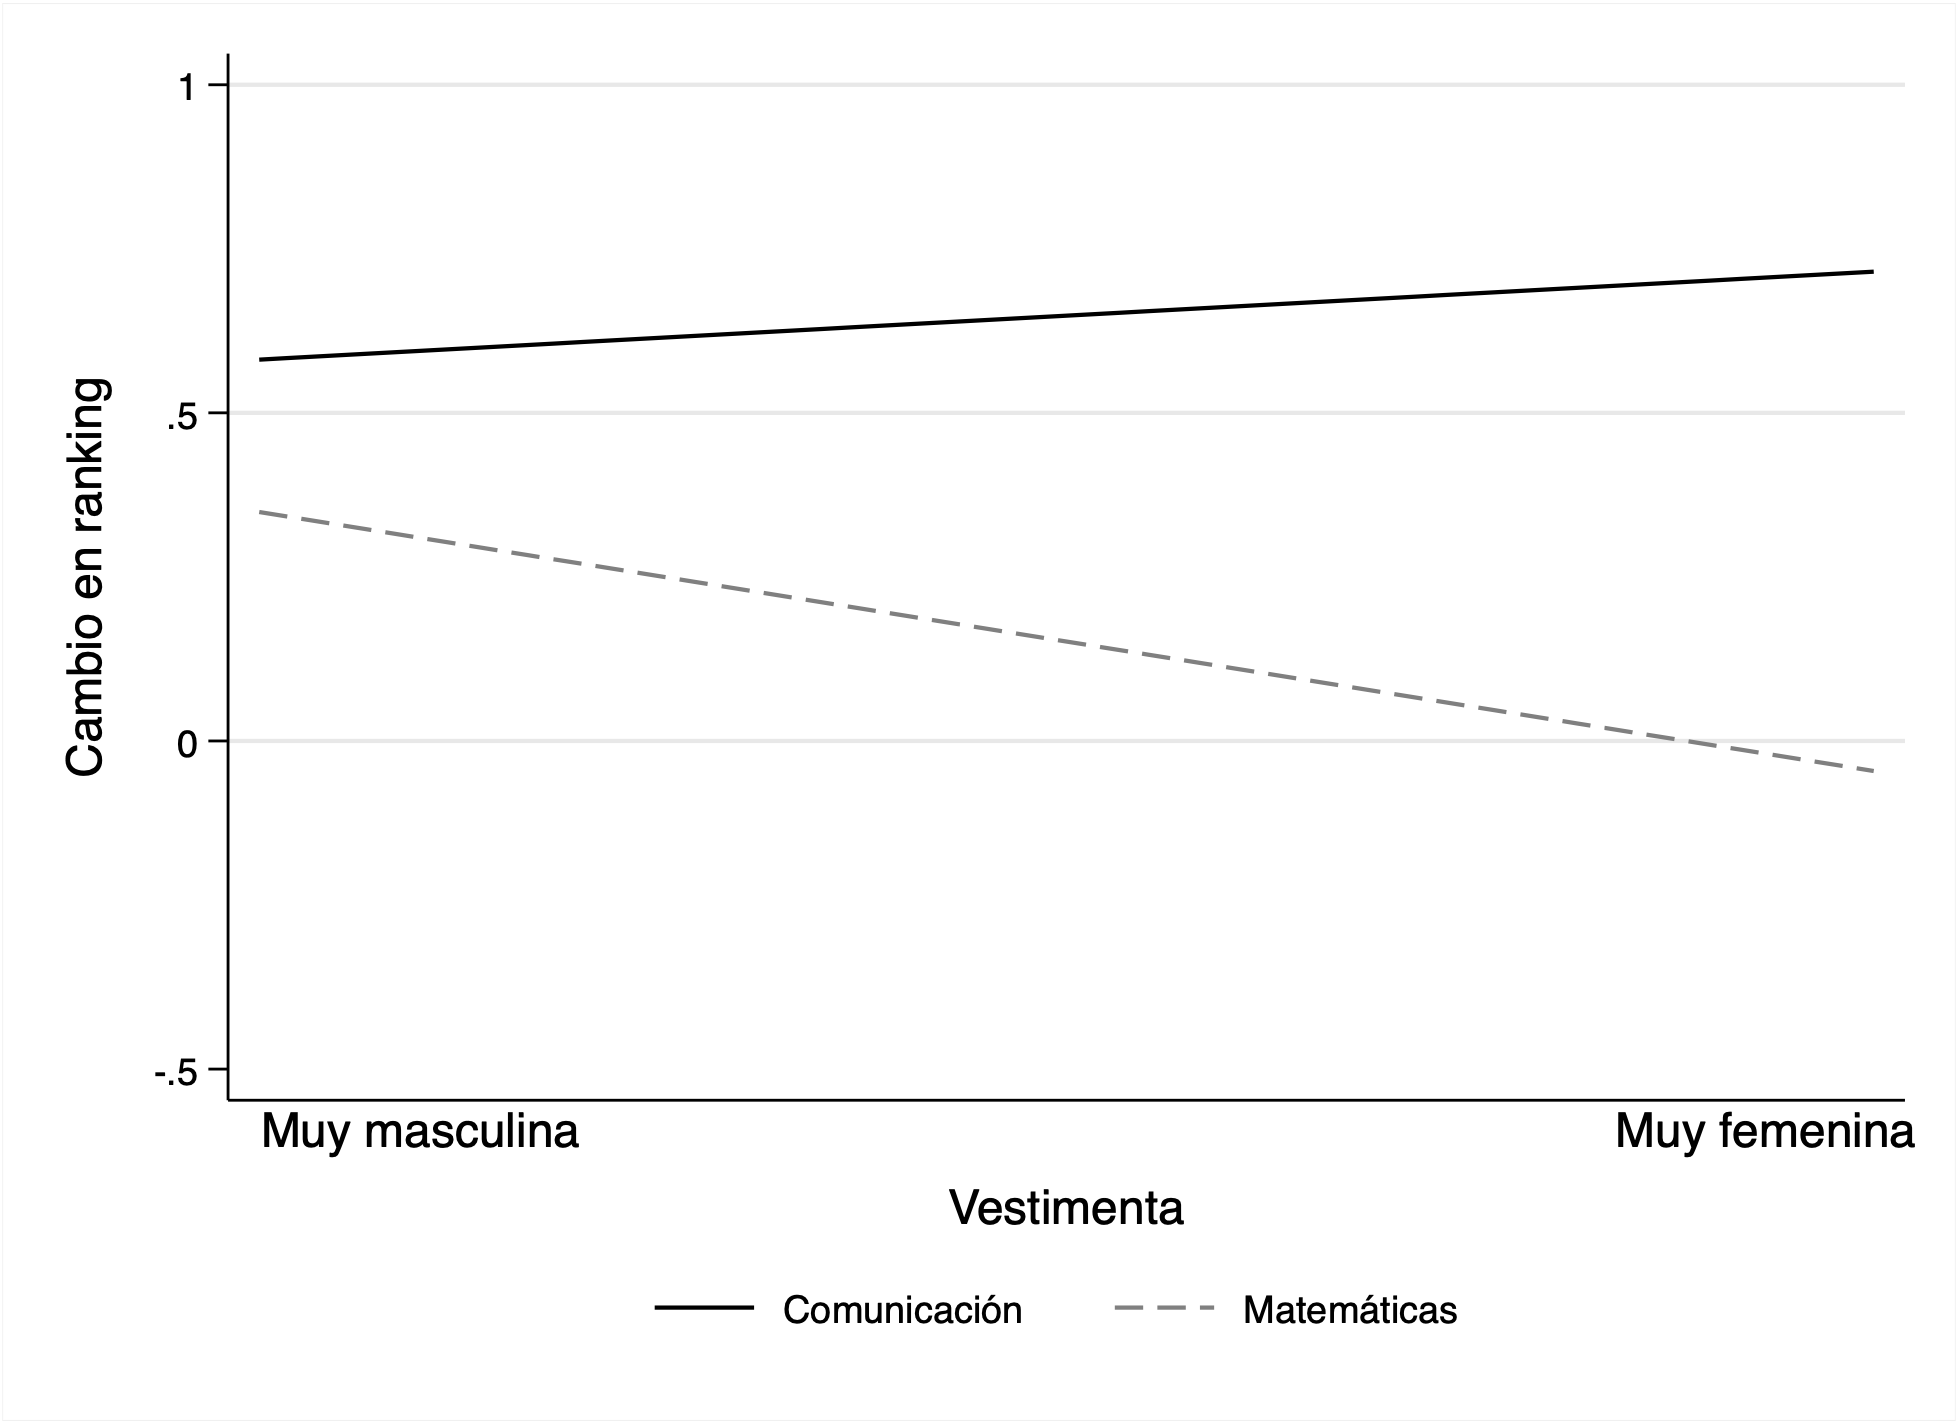
\includegraphics[width=7.8cm]{Images/h1_predicted_rank_score.png}
    \end{subfigure}
    \begin{minipage}{0.245\textwidth}
        
    \end{minipage}
    \centering
    \begin{subfigure}[t]{0.49\textwidth}
        \centering
        \caption{Rankers femeninos}
        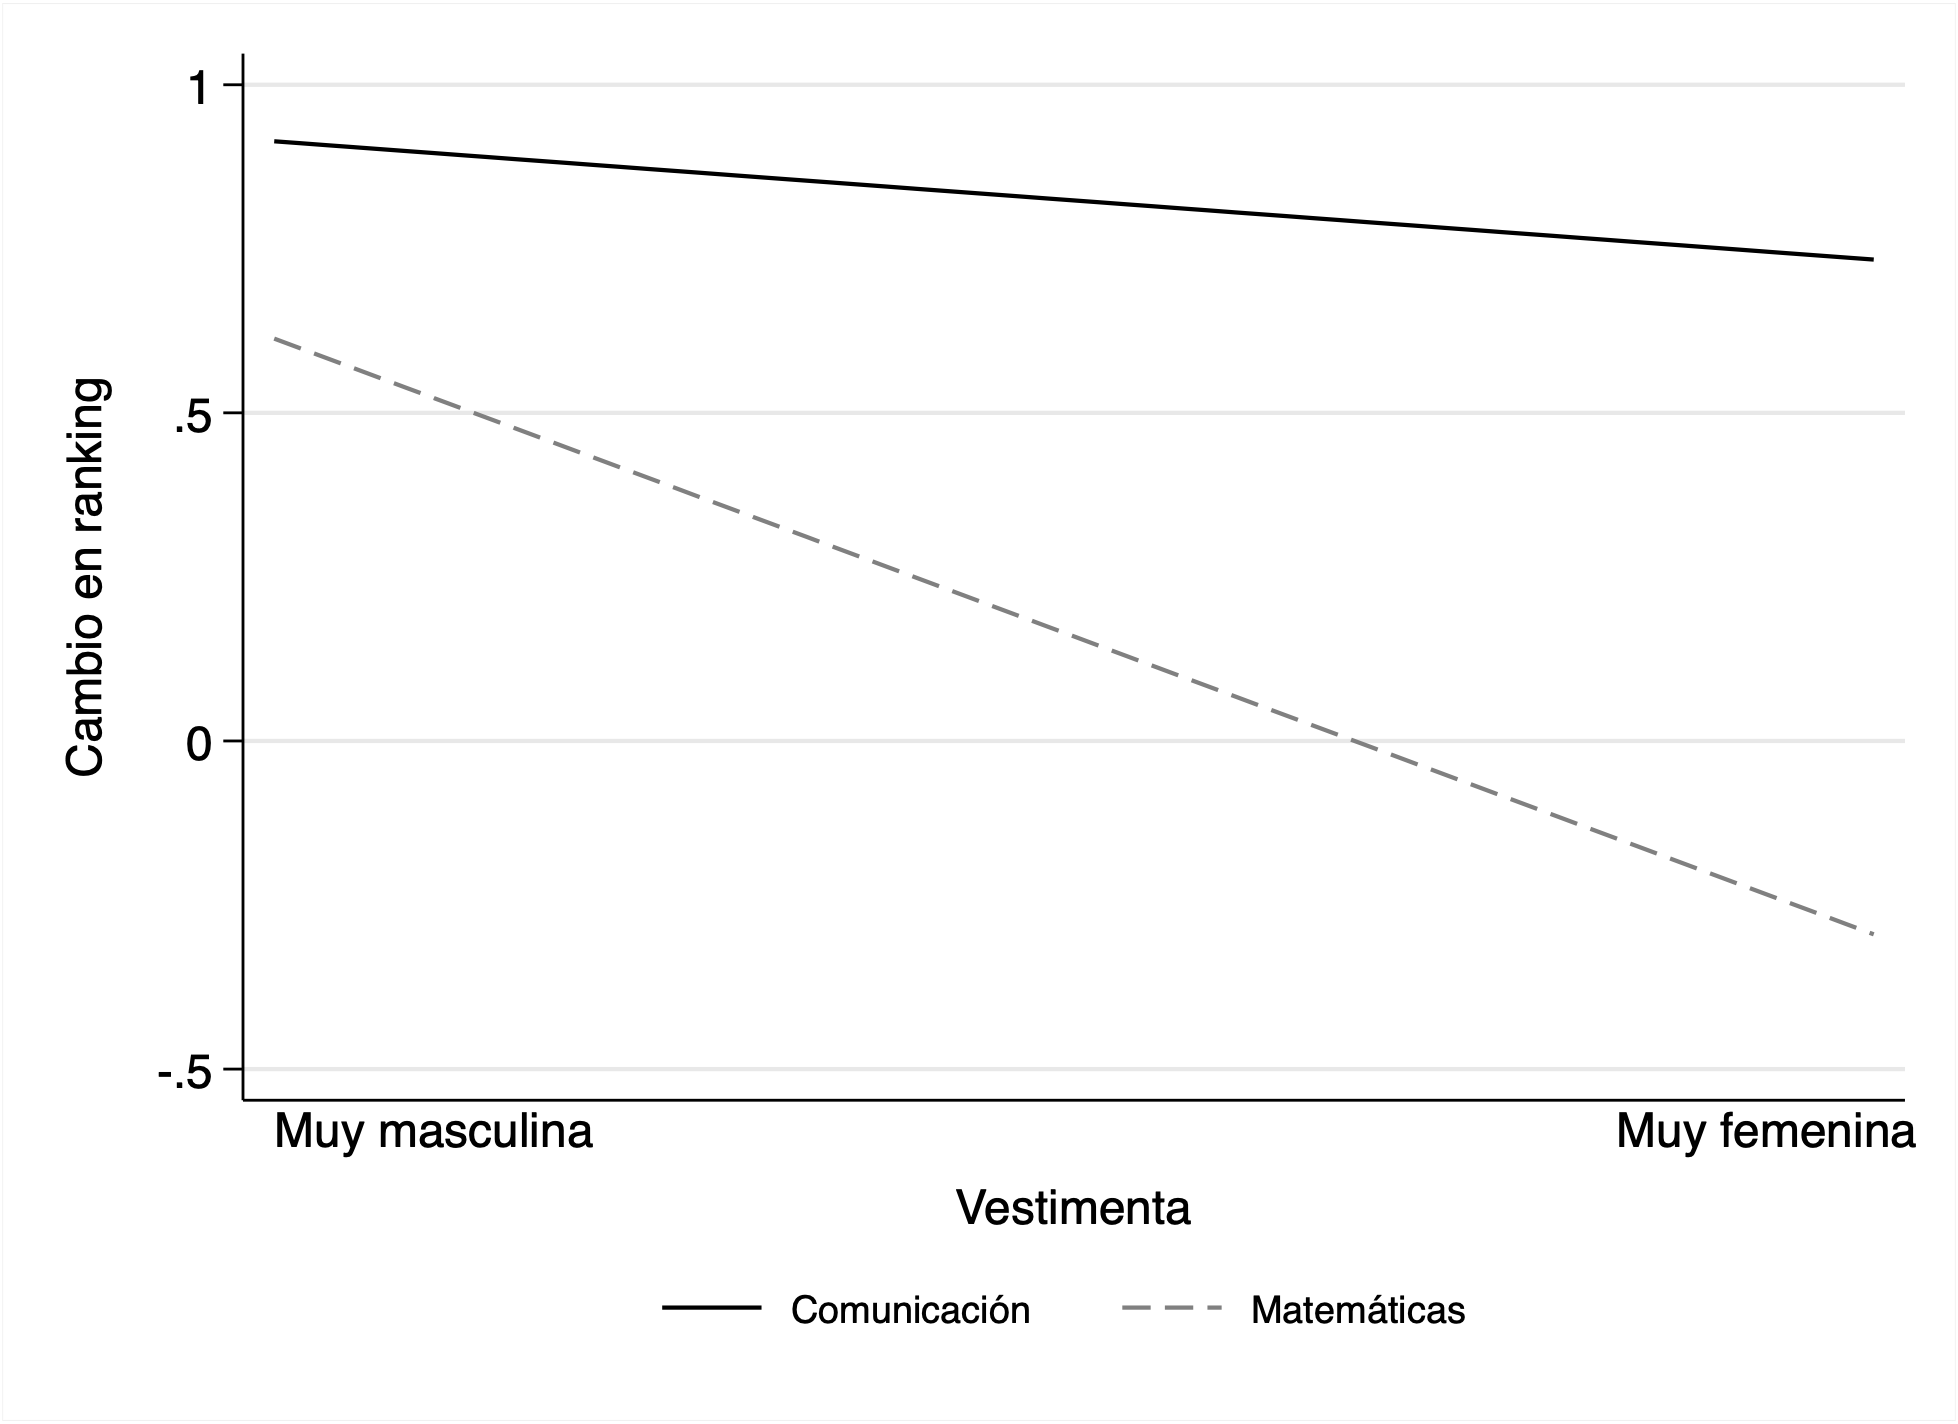
\includegraphics[width=7.8cm]{Images/h2_predicted_rank_score_fem.png}
    \end{subfigure}
    \begin{subfigure}[t]{0.49\textwidth}
        \centering
        \caption{Rankers masculino}
        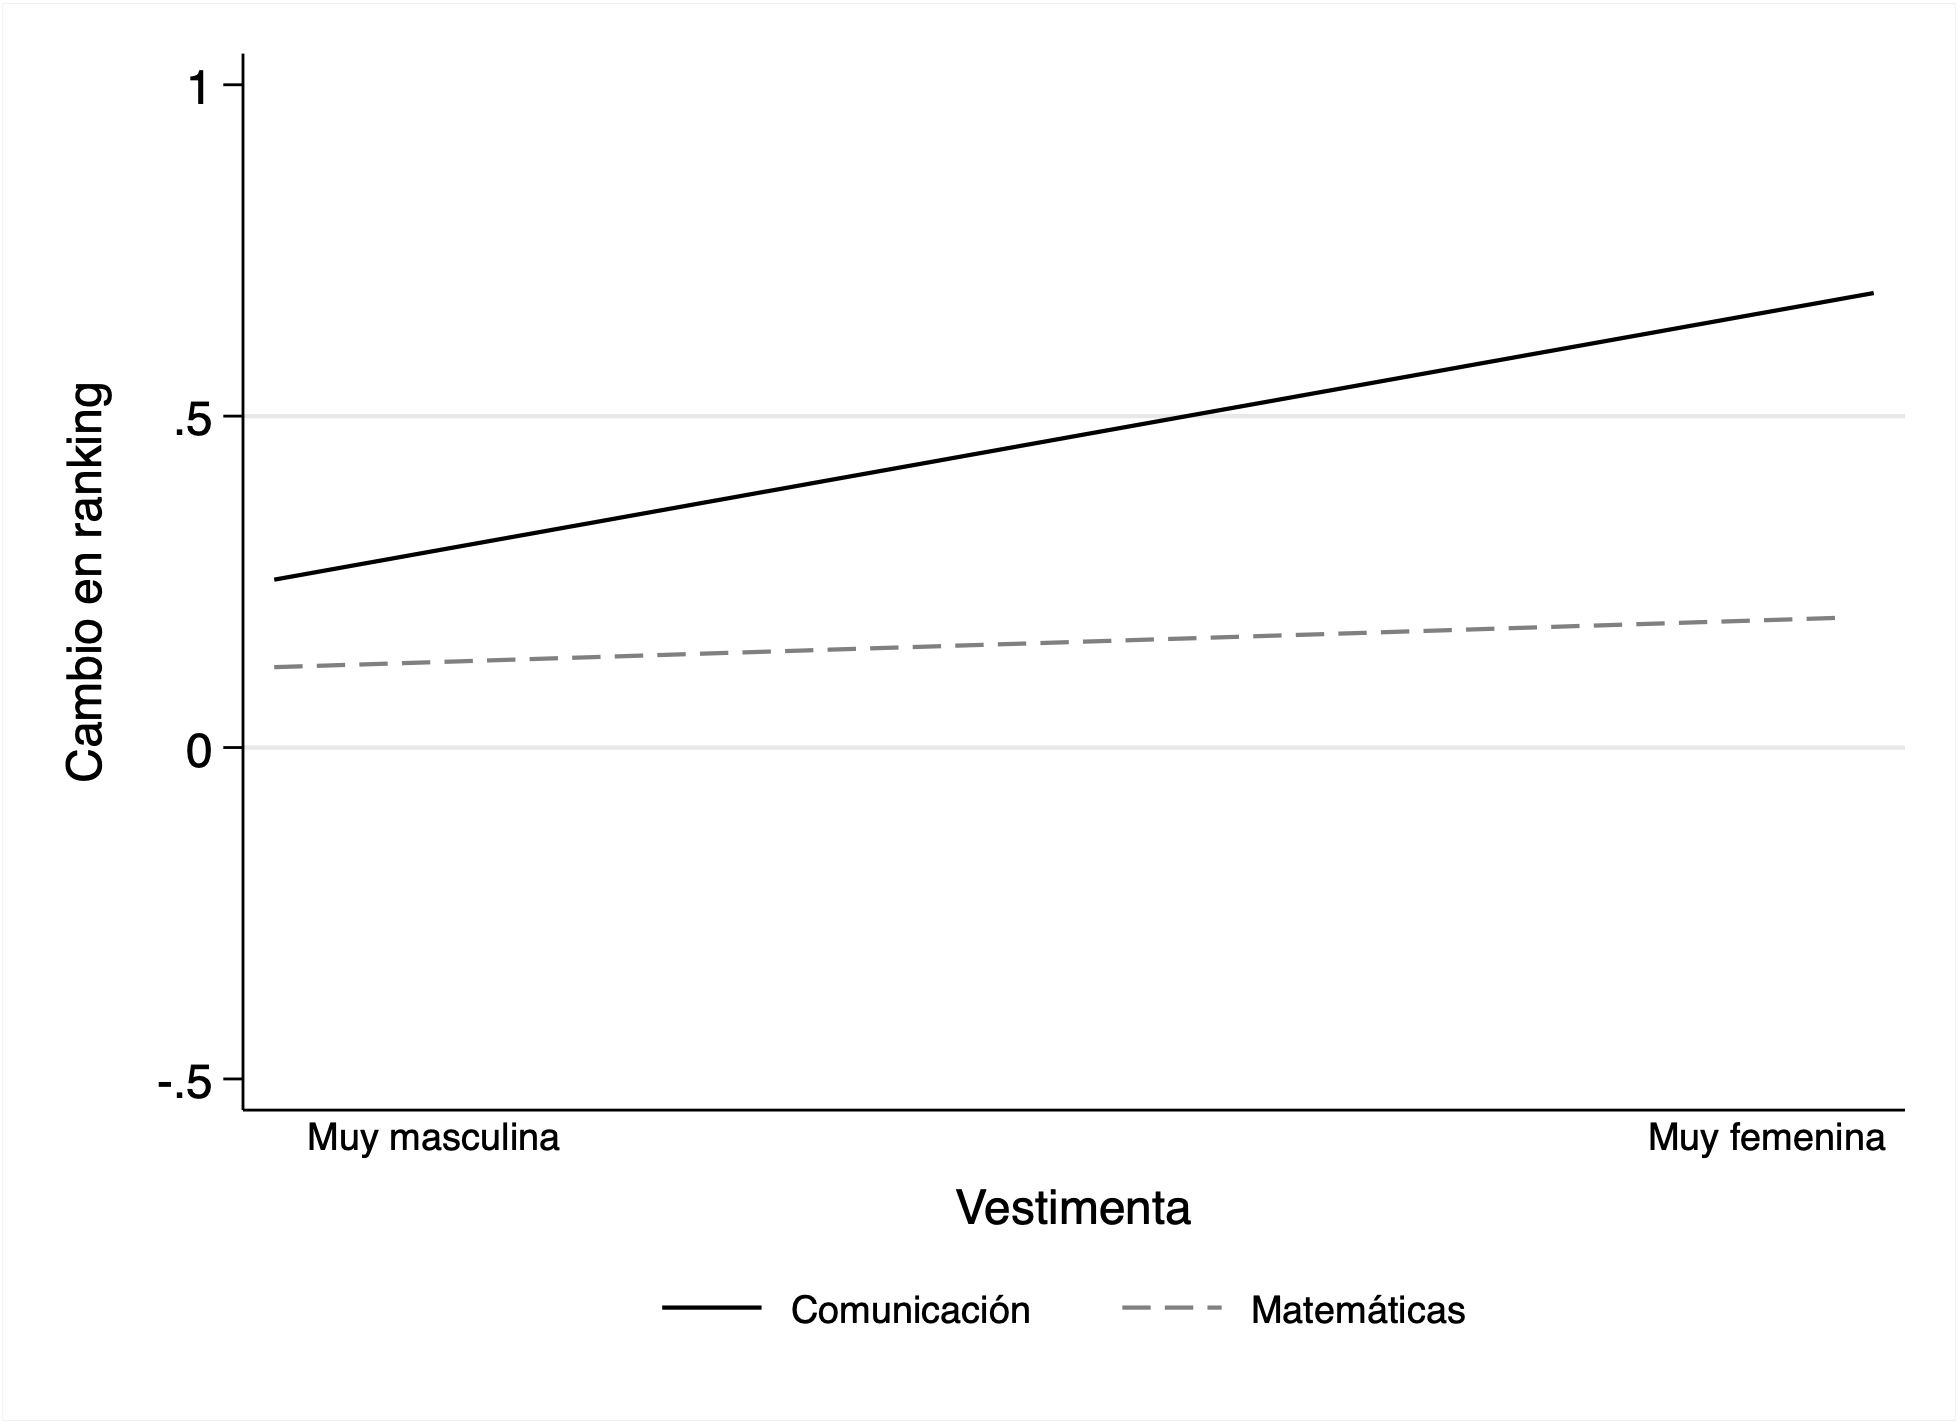
\includegraphics[width=7.8cm]{Images/h2_predicted_rank_score_masc.png}
    \end{subfigure}
    \begin{singlespace}
    \floatfoot{\footnotesize{\textit{Nota:} Gráfica del cambio esperado en el orden del listado por combinación de expresiones de género. La  gráfica (a) está construida a partir de los resultados de la estimación por MCO de la ecuación 1. Las gráficas (b) y (c) están construidas a partir de la estimación por MCO de la ecuación 1, agregando la interacción entre el género de la persona que organiza los perfiles y las variables de expresiones de género (vestimenta, habilidad y habilidad*vestimenta). Las gráficas corresponden al valor predicho del ranking (controlando por la edad promedio, una aspiración familiar, haber nacido en Bogotá, y haber tenido una posición inicial de cuatro) corregido por la posición inicial (ranking predicho menos posición inicial (cuatro)). }\par}
    \end{singlespace}
\end{figure}

Lo que resulta interesante es que dentro de las personas cuya habilidad principal era la comunicación, las personas con una vestimenta femenina recibieron un \textit{ranking} 0.06d.e. más alto de las que tenían una vestimenta masculina. De manera similar, dentro de las personas que reportaron ser más hábiles en matemáticas, las personas que eligieron una vestimenta masculina, en promedio estuvieron 0.17d.e. más arriba en el \textit{ranking} que las personas con una vestimenta femenina. 

Por otra parte, en la población agregada, la diferencia entre el el \textit{ranking} que recibió una persona más hábil comunicándose y el \textit{ranking} que recibió una persona más hábil en matemáticas, aumenta a medida que la vestimenta es más femenina. Para una persona que eligió una vestimenta muy masculina, pasar de reportar como habilidad principal las matemáticas a reportar la comunicación aumentaba su \textit{ranking} en 0.1d.e. Mientras que para una persona con vestimenta muy femenina, pasar de reportar como habilidad principal las matemáticas a reporta la comunicación, aumenta su \textit{ranking} en 0.33d.e. 

\begin{table}[ht]
    \centering
    \caption{Diferencia en \textit{ranking} por combinaciones de expresiones de género y tipo de \textit{ranker}}
    \begin{subtable}{\textwidth}
        \centering
        \caption{Todos}
        \fontsize{9.5}{12}\selectfont {
        \begin{tabular}{cccccc}\hline \hline
                                         &	\multicolumn{2}{c}{\textit{Comunicación}}   &   
                                         &	\multicolumn{2}{c}{\textit{Matemáticas}}	\\ \cmidrule{2-3} \cmidrule{5-6}
                                         &  \textit{Vest. F}    &   \textit{Vest. M}    &   
                                         &  \textit{Vest. F}    &   \textit{Vest. M}    \\ \hline
        \textit{Vest. F \& Comunicación} &	-	                &   0.13                &   
                                         &   0.76               &  	0.37                \\
        \textit{Vest. M \& Matemáticas } &  -0.37	            &   -0.23	            &   
                                         &   0.39               &     -	                \\ \hline\hline
    \end{tabular}}
    \end{subtable}
    \begin{subtable}{\textwidth}
        \centering
        \vspace*{0.5cm}
        \caption{\textit{Ranker} femenino}
        \fontsize{9.5}{12}\selectfont {
        \begin{tabular}{cccccc}\hline \hline
                                         &	\multicolumn{2}{c}{\textit{Comunicación}}   &   
                                         &	\multicolumn{2}{c}{\textit{Matemáticas}}	\\ \cmidrule{2-3} \cmidrule{5-6}
                                         &  \textit{Vest. F}    &   \textit{Vest. M}    &   
                                         &  \textit{Vest. F}    &   \textit{Vest. M}    \\ \hline
        \textit{Vest. F \& Comunicación} &  -	                &   -0.18               &   
                                         &  1.03                &   0.12                \\
        \textit{Vest. M \& Matemáticas } &  -0.12	            &   -0.30	            &   
                                         &  0.91                &   -	                \\ \hline\hline
        \end{tabular}}
    \end{subtable}
    \begin{subtable}{\textwidth}
        \centering
        \vspace*{0.5cm}    
        \caption{Ranker masculino}
        \fontsize{9.5}{12}\selectfont {
        \begin{tabular}{cccccc}\hline \hline
                                         &	\multicolumn{2}{c}{\textit{Comunicación}}   &   
                                         &	\multicolumn{2}{c}{\textit{Matemáticas}}	\\ \cmidrule{2-3} \cmidrule{5-6}
                                         &  \textit{Vest. F}    &   \textit{Vest. M}    &   
                                         &  \textit{Vest. F}    &   \textit{Vest. M}    \\ \hline
        \textit{Vest. F \& Comunicación} &	-	                &   0.43                &   
                                         &  0.49                & 	0.56                \\
        \textit{Vest. M \& Matemáticas}  &  -0.56	            &   -0.13	            &   
                                         &  -0.08               &   -	                \\ \hline\hline
        \end{tabular}}
    \end{subtable}
    \begin{threeparttable}
    \begin{tablenotes}
    \footnotesize{
    \item Nota: Vest. F corresponde a una vestimenta muy femenina (1.5d.e arriba del promedio) y Vest. M corresponde a una vestimenta muy masculina (1.5d.e abajo del promedio). El valor corresponde a la fila menos la columna. Si el valor es positivo, es porque la combinación de expresiones de género de la fila tiene un mejor ranking que la combinación de la columna. Por ejemplo, una persona con todas vestimenta y habilidad femeninas en promedio está 0.13 puestos más arriba en el ranking que una que tiene una vestimenta femenina y habilidad masculina (Panel (a), la fila superior, segunda columna).}
    \end{tablenotes}
    \end{threeparttable}
    \label{tab:hypothesis_tables}
\end{table}

\begin{result}
Condicional en la habilidad, sugestivamente, existe una mayor disposición a interactuar con las personas que señalizan que cumplen la norma social, especialmente cuando señaliza una identidad femenina. 
\end{result}

 
Ahora bien, cuando el ranker era de identidad femenina, el efecto de cambiar la vestimenta de muy femenina a muy masculina, condicional a que la habilidad principal eran las matemáticas, es de un aumento de 0.4 d.e. en el \textit{ranking}. Por el contrario, el mismo cambio en vestimenta, cuando la habilidad principal de sus pares era la comunicación, baja el ranking en 0.08d.e. En resumen, los \textit{rankers} de identidad femenina presentaron una preferencia por trabajar con pares que tenían vestimenta masculina y su habilidad principal era la comunicación, y el tipo de persona con la que estaban menos dispuestos a interactuar era con aquellos que tenían vestimenta muy femenina y su habilidad principal eran las matemáticas. 

\begin{table}[htbp]
    \centering
    \caption{Diferencia en ranking por género del ranker}
    \label{tab:Diffs}

    \fontsize{9.5}{12}\selectfont {
    \begin{tabular}{ccccc}\hline \hline
          \multicolumn{2}{c}{\textit{Comunicación}} &   
        & \multicolumn{2}{c}{\textit{Matemáticas}}	\\ \cmidrule{1-2} \cmidrule{4-5}
          \textit{Vest. F}  &   \textit{Vest. M}    &   
        & \textit{Vest. F}  &   \textit{Vest. M}    \\ \hline
	      0.05	            &   0.66                &
	    & -0.49             &   0.49                \\ \hline \hline
    \end{tabular}}

    \begin{threeparttable} 
    \begin{tablenotes}
    \scriptsize{
    \item Nota: Vest. F corresponde a una vestimenta muy femenina (1.5d.e arriba del promedio) y Vest. M corresponde a una vestimenta muy masculina (1.5d.e abajo del promedio). En el panel (a) el valor corresponde a la diferencia entre la posición promedio que en la que una persona de identidad femenina a un perfil con esa combinación de expresiones de género y la posición promedio que una persona de identidad masculina le da a ese mismo perfil.} 
    \end{tablenotes}
    \end{threeparttable}
\end{table}

Cuando el \textit{ranker} era de identidad masculina, las personas con vestimenta femenina y hábiles comunicándose recibieron el mejor ranking. En esta submuestra, el efecto de pasar de tener una vestimenta muy masculina a tener una muy femenina, cuando la habilidad principal era la comunicación, es de 0.19d.e. Un efecto tres veces más grande que el de la muestra completa. Por el contrario, cuando la habilidad principal eran las matemáticas, los \textit{rankers} de identidad masculina fueron prácticamente indiferentes de la vestimenta. 


\begin{result}
Existen diferencias en la disposición a interactuar de \textit{rankers} femeninos y masculinos ante diferentes combinaciones de expresiones de género. 
\end{result}

